\documentclass[11pt]{article}

\usepackage{extras} % Se extras.sty
\usepackage{tikz}
\usepackage{graphicx}


\begin{document}
\begin{titlepage}
\begin{center}

{\Large\bfseries TSEA56 - Kandidatprojekt i elektronik \\ LIPS Förstudie: Sensor}

\vspace{5em}

Version 0.1

\vspace{5em}
Grupp 4 \\
\begin{tabular}{rl}
Wasteson, Emil&\verb+emiwa068+
\\
Inge, Zimon&\verb+zimin415+
\\
\end{tabular}

\vspace{5em}
\today

\vspace{16em}
Status
\begin{longtable}{|l|l|l|} \hline

Granskad & - & - \\ \hline
Godkänd & - & - \\ \hline
 
\end{longtable}

\end{center}
\end{titlepage}

\pagebreak
\begin{center}

\section*{PROJEKTIDENTITET}
2016/VT, Undsättningsrobot Gr. 4

Linköpings tekniska högskola, ISY
\vspace{5em}
\begin{center}

\begin{tabular}{|l|l|l|l|} \hline
\textbf{Namn} & \textbf{Ansvar} & \textbf{Telefon} & \textbf{E-post}  \\ \hline 
Isak Strömberg (IS) & Projektledare & 073-980 38 50 & isast763@student.liu.se \\ \hline
Olle Hynén Ulfsjöö (OHU)& Dokumentansvarig & 070-072 91 84 & ollul666@student.liu.se \\ \hline
Emil Wasteson (EW) & Hårdvaruansvarig & 076-836 61 66 & emiwa068@student.liu.se \\ \hline
Elena Tronje (ET) & Mjukvaruansvarig & 072-276 92 93 & eletr654@student.liu.se \\ \hline
Zimon Inge (ZI)& Testansvarig & 070-171 35 18 & zimin415@student.liu.se \\ \hline
Lovisa Gustafsson (LG) & Leveransansvarig & 070-210 32 53 & lovgu777@student.liu.se \\ \hline
\end{tabular}

\end{center}

E-postlista för hela gruppen: isast763@student.liu.se

\vspace{5em}
Kund: ISY, Linköpings universitet \\
tel: 013-28 10 00, fax: 013-13 92 82 \\
Kontaktperson hos kund: Mattias Krysander \\
tel: 013-28 21 98, e-post: matkr@isy.liu.se \\

\vspace{5em}
Kursansvarig:  Tomas Svensson\\
tel: 013-28 13 68, e-post: tomass@isy.liu.se \\
Handledare: Peter Johansson \\
tel: 013-28 13 45, e-post: peter.a.johansson@liu.se
\end{center}
\pagebreak

\tableofcontents

\pagebreak
\section*{Dokumenthistorik}
\begin{table}[h]
\begin{tabular}{|l|l|l|l|l|} \hline

\textbf{Version} & \textbf{Datum} & \textbf{Utförda förändringar} & \textbf{Utförda av} & \textbf{Granskad} \\ \hline
0.1 & - &  Första utkastet & Grupp 4 & - \\ \hline
\end{tabular}
\end{table}

\pagebreak
\pagenumbering{arabic}

\begin{flushleft}

\section{Inledning}
I dagsläget finns det en mängd olika sensorer, alla med för- respektive nackdelar. Vilken sensor som är bäst beror ofta på vilket syfte som ska uppfyllas och vilka resurser som finns att tillgå. Att en undsättningsrobot som ska hitta nödställda har sensorer som gör det enkelt att identifiera sitt mål är en fråga om liv och död. Därav finns det ett stort behov av att öka kunskapen om sensorer, samt dess möjligheter och begränsningar.

\pagebreak

\section{Problemformulering}

\subsection{Syfte}
Syftet med denna rapport är att undersöka vilka sensorer som är relevanta för undsättningsroboten i sitt uppdrag. Syftet är fortsättningsvis att redogöra för en implementation av de sensorer som finnes intressanta för undsättningsrobotens ändamål.


\subsection{Frågeställningar}
Nedan följer de huvudsakliga frågeställningar vilka har för avsikt att behandlas i denna rapport:

\begin{itemize}
\item{Vilka sensorer finns det som stöd för att roboten ska kunna utföra sitt uppdrag? Hur fungerar dessa? Finns det olika typer?}
\item {Vilka sensorer är lämpliga att använda till projektet?}
\item{Hur kan dessa implementeras? }
\end{itemize}

\pagebreak

\section{Kunskapsbas}
I följande avsnitt följer en beskrivning av olika typer av sensorer.

\subsection{Kapacitiv sensor}
Den kapacitiva sensorn är en sensor som använder sig av kapacitans (C) för att identifiera ett önskat material. Sensorn består av en platta med arean A och kan detektera alla objekt som har en relativ kapacivitet som skiljer sig från luft, bland annat plast, olika metaller, vätskor och hud. När avståndet (d) mellan objektet och sensorn minskar så ökar kapacitansen enligt Ekvation 1, där  är en konstant som beror av materialets relativa kapacivitet. 

I Figur 4 illustreras hur kapacitansen ändras när objektet (fingret) närmar sig sensorn och hur kapacitansändringen med hjälp av en AD-omvandlare görs om till en digital signal. 


http://www.ti.com/lit/an/snoa927/snoa927.pdf

http://www.fujitsu.com/downloads/MICRO/fme/articles/fujitsu-whitepaper-capacitive-touch-sensors.pdf

http://www.analog.com/library/analogDialogue/archives/40-10/cap_sensors.html



\subsection{Ljussensor}
Ljussensorn (även kallad fotocell) omvandlar infallande ljus till elektrisk ström. Strömstyrkan varierar beroende ljusets styrka, varför en ljussensor är användbar vid detektering av konstraster på exempelvis en yta.

\subsubsection{Reflektorfotocell}
En reflektorfotocell är en typ av ljussensor som detekterar förändringar i ljusintensiteten. Den typiska reflektorfotocelnne består av en ljuskälla, en motagare, en signalkonverterare och slutligen en förstärkare.

http://www.automation.com/library/articles-white-papers/sensors-sensing-technologies/fundamentals-of-photoelectric-sensors


\subsubsection{Direktavkännare}

\subsubsection{Sändare/mottagare}

\subsubsection{IR-sensor}
En IR-sensor är en tillämpning av en ljussensor som endast registrerar önskade våglängder i det infraröda spektrumet. I figur 1 illustreras hur en sensor, med hjälp av en LED-lampa som sänder ut strålning med samma våglängd som den sensorn uppfattar, kan avgöra om ett det finns ett objekt i sensorns riktning. Detekteras reflekterad strålning betyder det att ett föremål finns i sensorns riktning.

\begin{figure}[htbp]
	\centering
	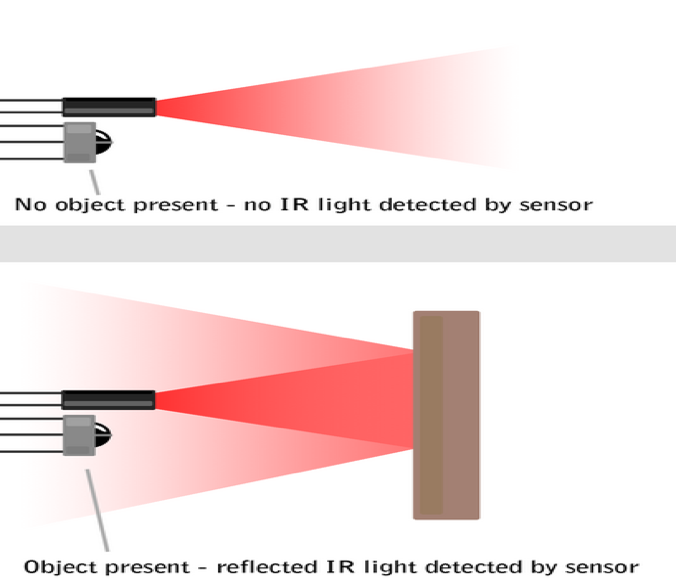
\includegraphics[scale=0.4]{Images/Laser}
	\caption{Illustration av lasersensor \label{Laser}}
\end{figure}

Det går även att använda som en avståndssensor, vilket illustreras i figur 2, genom att sensorn mäter vinkeln av det reflekterade ljuset som strålningen av LED-lampan ger upphov till. Detta ställer högre krav på sensorn, eftersom strålningen behöver vara skarpare.

\begin{figure}[htbp]
	\centering
	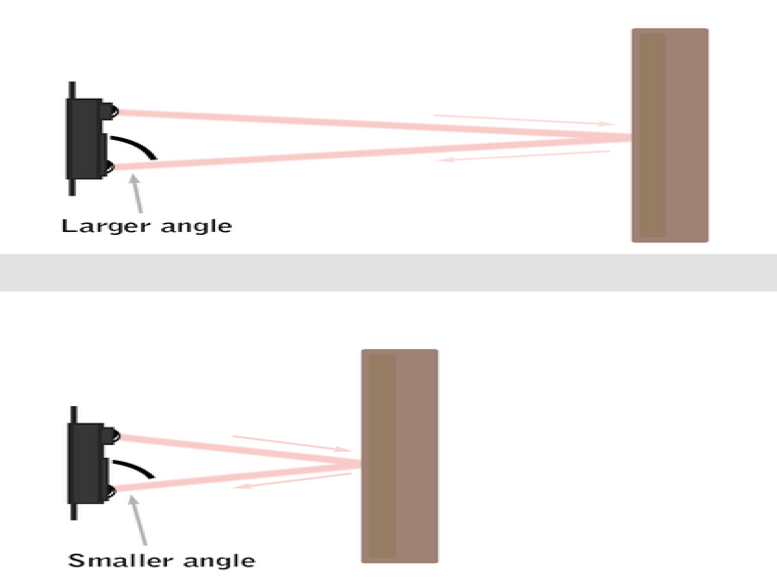
\includegraphics[scale=0.4]{Images/laser_angle}
	\caption{Vinkelmätning med lasersensor \label{laser_angle}}
\end{figure}

Ytterligare en möjlighet med en IR-sensor är att mäta hur ljusskillnader. Eftersom ljusa objekt reflekterar mer ljus än vad mörka gör kan sensorn reagera på reflektioner mot ett ljust objekt, men inte mot ett mörkt.



http://education.rec.ri.cmu.edu/content/electronics/boe/ir_sensor/1.html


\pagebreak
\section{Rapportens huvuddel, byt rubriknamn}
text

\section{Resultat och slutsatser}
text

\pagebreak
\addcontentsline{toc}{section}{Referenser}
\bibliographystyle{ieeetr}
\bibliography{references}

\pagebreak
\appendix
\section{First Appendix}

\end{flushleft}
\end{document}